\subsection{La ley de la gravitación de Newton y el movimiento de los planetas}
\textbf{Propósito:} Deducir las leyes de Kepler a partir de la ley de la gravitación universal de Newton. Para ello, se analiza el movimiento de una partícula de masa $m$ (un planeta) bajo la atracción de una partícula fija de masa $M$ mucho mayor (el sol).

\begin{figure}[htbp]
    \centering
    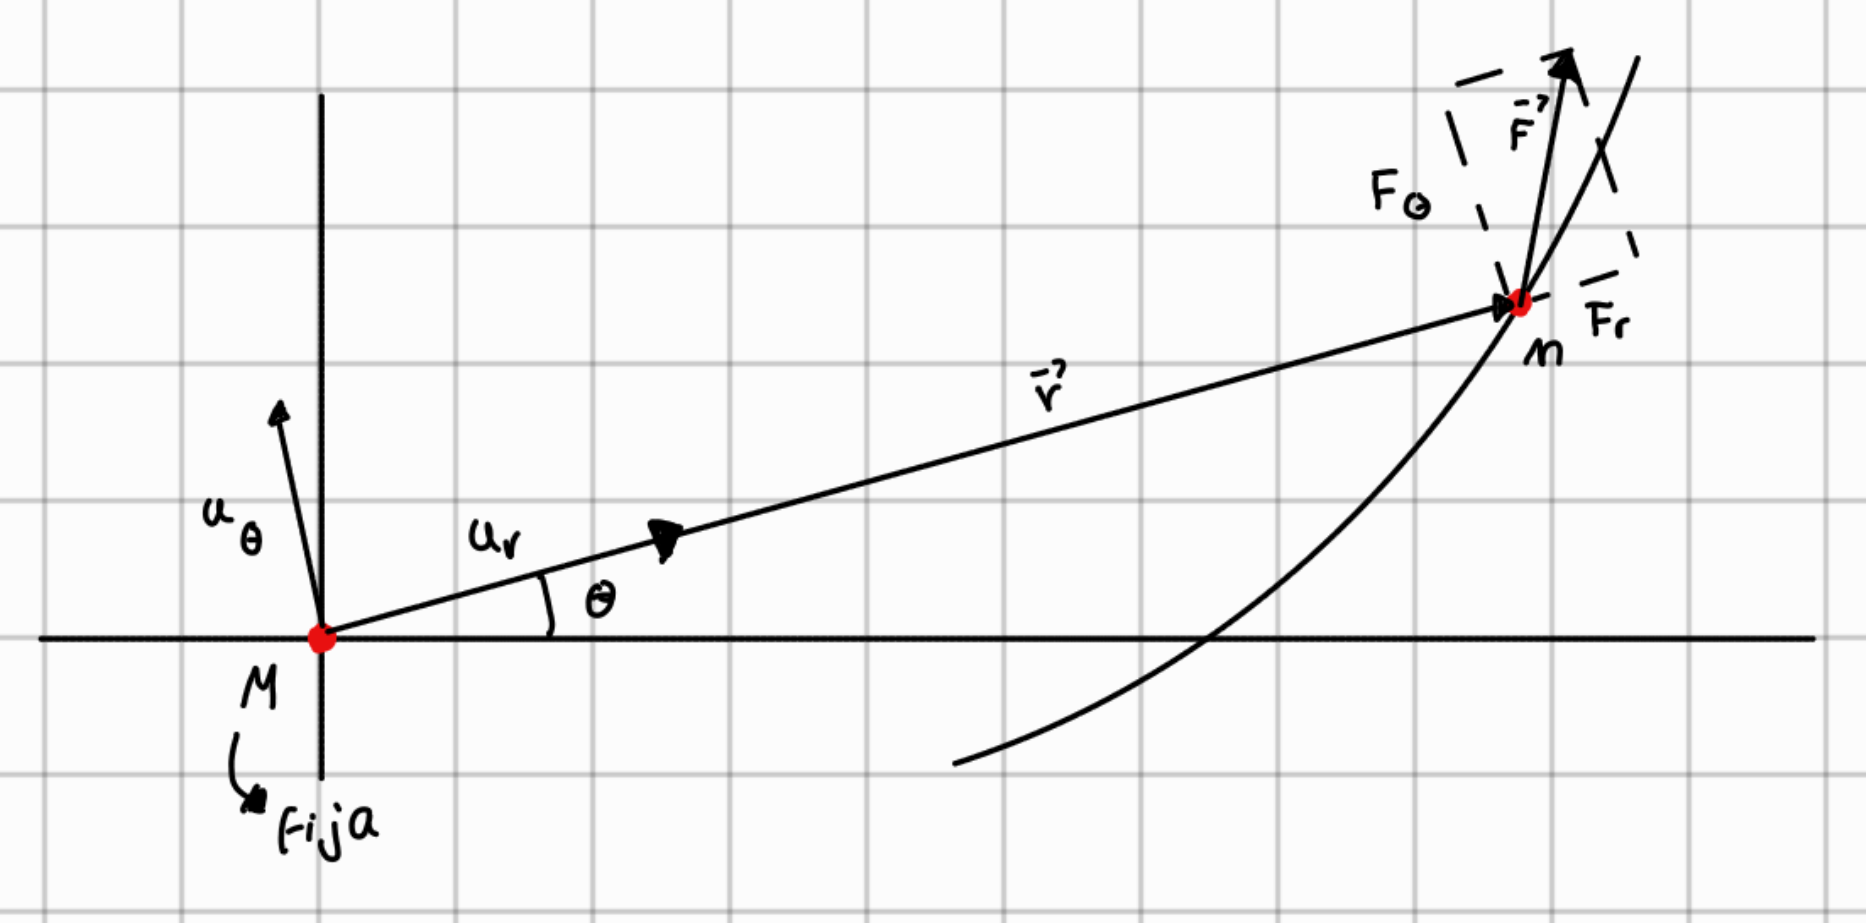
\includegraphics[width=0.8\textwidth]{./Sessions/Two-Body-Problem/Images/simmons-img1.png}
    \caption{Diagrama de cuerpo libre para el problema de dos cuerpos.}
    \label{fig:dcl_2cuerpos}
\end{figure}

En problemas de movimiento bajo una fuerza dirigida a un punto fijo, conviene descomponer los vectores en componentes radiales y perpendiculares a esta. El vector posición es:
\[ \vec{r} = r\vec{u}_r \]
cuyo vector unitario es:
\[ \vec{u}_r = \cos\theta \hat{i} + \sin\theta \hat{j} \]
y su vector perpendicular, en la dirección de $\theta$ creciente, es:
\[ \frac{d\vec{u}_r}{d\theta} = -\sin\theta \hat{i} + \cos\theta \hat{j} = \vec{u}_\theta \]
De la derivación se obtienen las relaciones esenciales:
\[ \frac{d\vec{u}_r}{d\theta} = \vec{u}_\theta \quad \text{y} \quad \frac{d\vec{u}_\theta}{d\theta} = -\vec{u}_r \]
Estas relaciones nos permiten obtener los vectores velocidad y aceleración.
\[ \vec{v} = \frac{d\vec{r}}{dt} = \frac{d}{dt}(r\vec{u}_r) = \frac{dr}{dt}\vec{u}_r + r\frac{d\vec{u}_r}{dt} \]
Por regla de la cadena, ya que $\vec{u}_r$ depende de $\theta$ y $\theta$ de $t$:
\[ \vec{v} = \frac{dr}{dt}\vec{u}_r + r\frac{d\vec{u}_r}{d\theta}\frac{d\theta}{dt} \]
\[ \vec{v} = \frac{dr}{dt}\vec{u}_r + r\frac{d\theta}{dt}\vec{u}_\theta \]
Y el vector aceleración, tras un cálculo directo a partir de $\vec{v}$, es:
\[ \vec{a} = \left[\frac{d^2r}{dt^2} - r\left(\frac{d\theta}{dt}\right)^2\right]\vec{u}_r + \left[r\frac{d^2\theta}{dt^2} + 2\frac{dr}{dt}\frac{d\theta}{dt}\right]\vec{u}_\theta \]
Si $\vec{F}$ es la fuerza que actúa sobre $m$, entonces $\vec{F} = F_r\vec{u}_r + F_\theta\vec{u}_\theta$.
Recordando la segunda ley de Newton, $\vec{F}=m\vec{a}$, se concluye que:
\begin{align}
    m\left(r\frac{d^2\theta}{dt^2} + 2\frac{dr}{dt}\frac{d\theta}{dt}\right) &= F_\theta \tag{1} \\
    m\left(\frac{d^2r}{dt^2} - r\left(\frac{d\theta}{dt}\right)^2\right) &= F_r \tag{2}
\end{align}
Estas ecuaciones diferenciales gobiernan el movimiento de la partícula, sea cual sea la naturaleza de la fuerza.

\subsection{Fuerzas centrales y segunda ley de Kepler}
Se dice que $\vec{F}$ es una fuerza central si está siempre dirigida a lo largo de la línea que une la partícula con el origen, es decir, si no tiene componente perpendicular, $F_\theta=0$. Bajo esta hipótesis, la ecuación (1) queda como:
\[ r\frac{d^2\theta}{dt^2} + 2\frac{dr}{dt}\frac{d\theta}{dt} = 0 \]
Multiplicando por $r$, la expresión se puede reconocer como la derivada de un producto:
\[ \frac{d}{dt}\left(r^2\frac{d\theta}{dt}\right) = 0 \]
Integrando ambos lados, se obtiene que:
\begin{equation} r^2 \frac{d\theta}{dt} = h \tag{3} \end{equation}
donde $h$ es una constante de integración. Si $A=A(t)$ es el área barrida por el radio vector, el diferencial de área es $dA = \frac{1}{2}r^2d\theta$. La tasa con que se barre el área es:
\[ \frac{dA}{dt} = \frac{1}{2}r^2\frac{d\theta}{dt} = \frac{h}{2} \]
Como $h$ es constante, la velocidad areolar también lo es. Al integrar entre dos instantes de tiempo, se obtiene que $A(t_2) - A(t_1) = \frac{h}{2}(t_2-t_1)$. Esta es la \textbf{Segunda Ley de Kepler}: el radio vector barre áreas iguales en intervalos iguales de tiempo\footnote{Kepler (1571-1630) destiló sus tres leyes tras trabajar incesantemente durante veinte años con la gran cantidad de datos observacionales heredados del astrónomo danés Tycho Brahe.}.

\subsection{Fuerzas gravitacionales centrales y primera ley de Kepler}
Ahora se especializa el análisis para una fuerza central atractiva cuya magnitud sigue la ley de la gravitación de Newton:
\[ F_r = -G\frac{Mm}{r^2} = -\frac{km}{r^2} \]
donde $k=GM$. La ecuación (2) pasa a ser:
\begin{equation} \frac{d^2r}{dt^2} - r\left(\frac{d\theta}{dt}\right)^2 = -\frac{k}{r^2} \tag{4} \end{equation}
El siguiente paso es obtener la ecuación de la órbita en forma polar $r=f(\theta)$, para lo cual se debe eliminar el tiempo $t$ y considerar $\theta$ como la variable independiente. Usando la ecuación (3) en la (4):
\begin{equation} \frac{d^2r}{dt^2} - \frac{h^2}{r^3} = -\frac{k}{r^2} \tag{5} \end{equation}
El libro de Simmons describe este paso como "difícil de motivar, ya que requiere considerable ingenio técnico". La presencia de potencias de $1/r$ sugiere el cambio de variable $z=1/r$. Se expresa $\frac{d^2r}{dt^2}$ en términos de $z$ y $\theta$:
\[ \frac{dr}{dt} = \frac{d}{dt}\left(\frac{1}{z}\right) = -h\frac{dz}{d\theta} \]
\[ \frac{d^2r}{dt^2} = -h^2z^2\frac{d^2z}{d\theta^2} \]
Al insertar esta expresión en (5) y sustituir $r=1/z$, queda:
\[ -h^2z^2\frac{d^2z}{d\theta^2} - h^2z^3 = -kz^2 \]
que se simplifica a la EDO lineal:
\[ \frac{d^2z}{d\theta^2} + z = \frac{k}{h^2} \]
La solución general es inmediata:
\begin{equation} z = A\sin\theta + B\cos\theta + \frac{k}{h^2} \tag{6} \end{equation}
Por simplificar, se desplaza el eje polar de modo que $r$ sea mínimo (perihelio) cuando $\theta=0$. Esto implica que $z$ es máximo, y por tanto $\frac{dz}{d\theta}|_{\theta=0}=0$, lo cual fuerza a que $A=0$. Despejando $r=1/z$:
\[ r = \frac{h^2/k}{1 + (Bh^2/k)\cos\theta} \]
Si se define la excentricidad $e = Bh^2/k$ (una constante positiva), la ecuación de la órbita se convierte en:
\begin{equation} r = \frac{h^2/k}{1+e\cos\theta} \tag{7} \end{equation}
Esta es la ecuación polar de una sección cónica con foco en el origen y excentricidad $e$. Puesto que los planetas permanecen en el sistema solar, sus órbitas son cerradas y la elipse ($e<1$) es la única posibilidad. Esto constituye la \textbf{Primera Ley de Kepler}: la órbita de cualquier planeta es una elipse con uno de sus focos en el Sol.

\subsection{Significado físico de la excentricidad y Tercera Ley de Kepler}
La energía total del sistema $E$ (cinética + potencial) es constante:
\[ E = \frac{1}{2}mv^2 - \frac{km}{r} \]
Se puede demostrar que la excentricidad depende directamente de la energía total del sistema:
\[ e = \sqrt{1 + E\left(\frac{2h^2}{mk^2}\right)} \]
Resulta claro que la naturaleza de la órbita queda completamente caracterizada por su energía total $E$. La órbita es una elipse si $E<0$, una parábola si $E=0$ y una hipérbola si $E>0$. Los planetas del sistema solar tienen energía negativa.

Para la Tercera Ley, se relaciona la dinámica con la geometría de la elipse. En astronomía, el semieje mayor $a$ se conoce como la distancia media. Es la semisuma de las distancias máxima y mínima de $r$. Un cálculo muestra que:
\[ a = \frac{h^2}{k(1-e^2)} \]
Usando la propiedad geométrica de la elipse $b^2 = a^2(1-e^2)$, se encuentra una relación para el semieje menor $b$:
\[ b^2 = \frac{h^2 a}{k} \]
Si $T$ es el período de la órbita, y el área de la elipse es $\pi ab$, de la segunda ley de Kepler se sigue que $\pi ab = hT/2$. Elevando al cuadrado y sustituyendo $b^2$:
\[ T^2 = \frac{4\pi^2 a^2 b^2}{h^2} = \frac{4\pi^2 a^2}{h^2}\left(\frac{h^2a}{k}\right) = \left(\frac{4\pi^2}{k}\right)a^3 \]
Como $k=GM$ es la misma constante para todos los planetas, se obtiene la \textbf{Tercera Ley de Kepler}: los cuadrados de los períodos de revolución de los planetas son proporcionales a los cubos de sus distancias medias.
